\documentclass[a4paper, 10pt, conference]{ieeeconf}
\usepackage[utf8]{inputenc}
\usepackage{graphicx}
\usepackage{amsmath}
\usepackage{amssymb}
\usepackage{url}
\usepackage{xcolor}
\usepackage{hyperref}
\usepackage{booktabs}
%
% ##########################
% include as many packages you need here
% ##########################
%



%
% ##########################
% Do not change this header
% ##########################
%
\title{WACV 2027 UPAR Challenge\\ \textit{Fact sheet}}
\begin{document}
\maketitle
This is the fact sheet's template for the \href{https://vap.aau.dk/rws/challenge/}{WACV 2027 UPAR Challenge}. Please fill out the following sections carefully in a scientific writing style. Then, send the compressed project (in \texttt{.zip} format), i.e., the generated PDF, \texttt{.tex}, \texttt{.bib} and any additional files to \url{upar.challenge@gmail.com}.
%
% end of the header
%------------------
%




% ##########################
% Next, you are asked to fill in the required information
% (please, do not remove/change any item)
% ##########################
%
\section{Team details}\label{teamdetails}
\begin{itemize}
    \item Team leader name: Muhammad Umar
    \item Username(s) on Codabench: \texttt{m\_umar}
    \item Team leader affiliation: FAST NUCES Karachi, BS Artificial Intelligence
    % \item Team leader address:
    % \item Team leader phone number:
    \item Team leader email: muhammad.umar26804@gmail.com
    \item Name of other team members (and affiliation): Raghib Rizwan Rabbani, Syed Fahad Faheem Shah (same affiliation as the team leader)
    \item Team website URL (if any): none
    \item Competition track (mark with X one single option)\footnote{If you participated in more than one competition track, you need to share with the organizers one fact sheet per track.}:
    \begin{itemize}
        \item (X) Track 1: Pedestrian Attribute Recognition.
        \item ( ) Track 2: Attribute-based Person Retrieval.
        \item ( ) Track 3: Human Pose Estimation.
    \end{itemize}
\end{itemize}
%
% end of 'Team details'
%------------------
%





% ##########################
% Next, you are asked to fill in the required information
% Here, you are free to add figures and tables, and expand the default sections to better explain your method and contributions.
% ##########################
%
\section{Contribution details}
%

\subsection{Title of the contribution}
\textbf{Averaging two fine-tuned CLIP ViT-L/14 image encoders for pedestrian attribute recognition under domain shift.}
We fine-tune the image tower of OpenAI CLIP ViT-L/14 with one sigmoid output per attribute, a loss that ignores attributes a dataset never annotates, and source-balanced sampling. Two such models, one trained by plain fine-tuning and one by linear probing followed by fine-tuning, are averaged in logit space and cut at 0.5. The model is shipped as plain PyTorch, so the submission needs only \texttt{torch}, \texttt{torchvision}, \texttt{numpy} and \texttt{Pillow}.


\subsection{Representative image / workflow diagram of the method}
\begin{figure}[h]
    \centering
    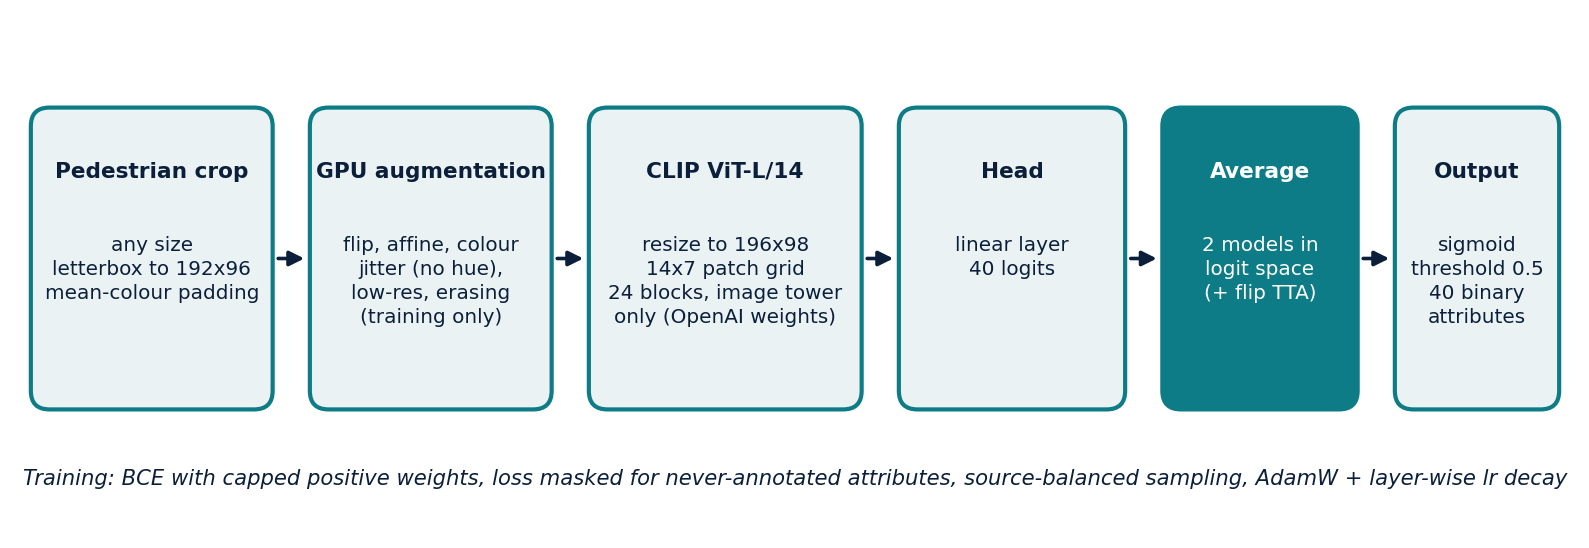
\includegraphics[width=\columnwidth]{pipeline.png}
    \caption{Pipeline of the final submission. Augmentation is used for training only; flip test-time augmentation is switched off automatically if the projected run time gets close to the 5-minute limit.}
    \label{fig:pipeline}
\end{figure}


\subsection{Detailed method description}
\textbf{Data and preprocessing.} We trained only on the organisers' data (Market1501, PA-100K and PETA, using the annotations of the UPAR dataset~\cite{Specker_2023_WACV,Cormier_2023_WACV,cormier2024upar}). Every crop is resized to fit inside $192\times 96$ pixels keeping its aspect ratio, centred on a canvas filled with the ImageNet mean colour (124, 116, 104), and stored once as \texttt{uint8}. The same function is used when building the training cache and inside \texttt{run.py}. The CLIP model then resizes this input bilinearly to $196\times 98$ pixels, which is a $14\times 7$ grid of $14\times 14$ patches, and normalises it with the CLIP mean and standard deviation.

\textbf{Model.} We use the image tower of OpenAI CLIP ViT-L/14~\cite{radford2021clip} (24 transformer blocks, width 1024, 16 heads, QuickGELU), a pretrained foundation model that was not trained for attribute recognition. The projection output (768-d) feeds a new linear layer with 40 outputs. The positional embedding is interpolated (bicubic) from the original $16\times16$ grid to $14\times 7$. The weights are loaded with \texttt{open\_clip} at training time only; for inference we ship a plain-PyTorch re-implementation of the tower (\texttt{upar\_clipvit.py}) whose output matches \texttt{open\_clip} (we checked the two agree before every run), so the container needs no extra package.

\textbf{Loss and sampling.} Each attribute is an independent binary problem, because about 11--12\% of PETA images have two upper-body colours. The loss is binary cross-entropy with a per-attribute positive weight $\min(10, n_{neg}/n_{pos})$. Attributes that a source never annotates (five colour attributes in Market1501, one in PETA) are masked out of the loss for that source, since a zero there means ``unknown''. Training batches are drawn with source-balanced sampling: the share of source $s$ is proportional to $n_s^{0.5}$, which lowers the weight of PA-100K (81\% of the training images) while keeping the larger sources dominant.

\textbf{Augmentation (on the GPU).} Horizontal flip (p=0.5); random affine (p=0.8; rotation up to $5^\circ$, zoom 0.9--1.1, shift up to 5\%); photometric changes (p=0.8; brightness, contrast and saturation up to 25\%); low-resolution simulation (p=0.2; down- and up-sampling with a scale of 0.4--0.8); random erasing (p=0.25; 2--15\% of the area, mean-coloured). We never change hue, shuffle channels or convert to grayscale, because 24 of the 40 attributes are colours.

\textbf{Optimisation.} AdamW (weight decay 0.05), batch size 64, mixed precision (fp16 with a gradient scaler), gradient clipping at 5, a linear warm-up of 0.5 epoch followed by a cosine schedule to $10^{-6}$. We use layer-wise learning-rate decay: the base learning rate is $10^{-5}$ for the last block and is multiplied by 0.85 for every block below it, the new head uses $10^{-3}$, and biases, norm parameters and embeddings get no weight decay. One epoch is 2048 steps of 64 images (about one pass over train+val). The two final models were trained on train+validation:
\begin{itemize}
    \item Model A: plain fine-tuning, 3 epochs, seed 0.
    \item Model B: linear probe then fine-tune: the first epoch trains only the head (backbone frozen), then all layers for 3 more epochs (4 epochs in total), seed 0.
\end{itemize}
Training one model took about 2 to 2.5 hours on a free Colab T4 GPU (about 37 minutes per epoch, 12.9~GB peak memory).

\textbf{Inference and post-processing.} Predictions of the two models are averaged in logit space, and an attribute is positive if the averaged probability is above 0.5 (no per-attribute thresholds, because threshold tuning on held-out sources gave no robust gain). The weights of the two models are stored in int8 with per-row scales (the decisions agreed with the fp16 weights on 99.94\% of validation outputs we checked), so the zip stays below 600~MB. \texttt{run.py} also supports horizontal-flip test-time augmentation and switches it off automatically when the projected time would exceed the 5-minute limit. If an image cannot be read, the training-set attribute frequencies are returned. The code never looks at the image name or folder.

\textbf{Model selection.} We chose the recipe with leave-one-source-out experiments: we trained on two sources and scored the third with the official metric, as a stand-in for the unseen test domain. On held-out PETA, ConvNeXt-Tiny reached 0.7474 and CLIP ViT-B/16 reached 0.786--0.788 (Challenge\_Avg). The L/14 models were trained directly on train+validation, with settings taken from those B/16 experiments. No test image was used for training, pseudo-labelling or tuning, and the leaderboard was only used to compare finished candidates.


\subsection{Challenge results}
Our last submission (the one shown on the leaderboard) is the two-model ensemble. We also list our earlier submissions.
\begin{table}[h]
\centering
\caption{Codabench results on the hidden test set (Track 1).}
\label{tab:results}
% \small
\resizebox{\columnwidth}{!}{%
\begin{tabular}{@{}llccc@{}}
\toprule
ID & Model & mA & Inst. F1 & Avg \\
\midrule
1001365 & Attribute-prior baseline & 0.5000 & 0.4910 & 0.4955 \\
1001777 & ConvNeXt-Tiny & 0.7302 & 0.7274 & 0.7288 \\
1002923 & CLIP ViT-B/16 (1 model) & 0.7693 & 0.7642 & 0.7668 \\
1003348 & CLIP ViT-B/16 (3 models) & 0.7676 & 0.7713 & 0.7694 \\
1006798 & CLIP ViT-L/14 (1 model) & 0.7802 & 0.7774 & 0.7788 \\
\textbf{1010210} & \textbf{CLIP ViT-L/14 (2 models), last} & \textbf{0.7754} & \textbf{0.7792} & \textbf{0.7773} \\
\bottomrule
\end{tabular}
}
\end{table}
The last submission (ID 1010210, user \texttt{m\_umar}) reached rank 42 on the leaderboard. The single L/14 model scored slightly higher (0.7788) but the difference to the ensemble is small; the ensemble was our final upload.


\subsection{Final remarks}
\textbf{Pros.} A large pretrained vision-language backbone transfers well to an unseen domain: switching from ConvNeXt-Tiny to CLIP was the largest single gain (about +0.04 on held-out PETA and +0.04 on the test set), and L/14 added about +0.01 over the B/16 ensemble. The pipeline is cheap to run (one L/14 with flip TTA took 141~s in total on the A10 runner) and the submission is dependency-free. The loss mask and capped weights handle the missing and rare labels without extra data.

\textbf{Cons.} The L/14 models were trained for only 3--4 epochs on a free GPU and without a held-out check, and most ablations use one seed, so differences below about 0.005 should be read as noise. Averaging two L/14 models did not improve over one. We did not use ensembles of different architectures, higher input resolution, CLIP text prompts or any test-time adaptation, which are natural next steps.


\section{Additional method details}
Please, reply if your challenge entry considered (or not) the following strategies and provide a brief explanation. For each question, mark with X one single option. \\

%
% mark with an X each question.
%
\begin{itemize}
%------------------------------------
\item \textbf{For the competition track associated with this fact sheet, you confirm that you have trained your model on the predefined datasets} (X) Yes, (~) No\\
%------------------------------------

%------------------------------------
\item \textbf{Did you use any pre-trained model:} (X)~Yes, (~)~No.\\ If yes, please detail (e.g., model architecture, training strategy, train data, etc.).\\
The image encoder of OpenAI CLIP ViT-L/14 (ViT-L-14 weights from \texttt{open\_clip}, pretrained on the WIT image-text pairs of OpenAI, not trained for attribute recognition). ConvNeXt-Tiny and ResNet-50 (torchvision, ImageNet-1k) were used only in earlier experiments and a first submission, not in the final entry. We fine-tuned all CLIP layers on the organisers' training and validation data.
%------------------------------------

%------------------------------------
\item \textbf{Did you use external data?} (~) Yes, (X) No\\
No external attribute data. The only external data is the one behind the pretrained CLIP weights described above.
%------------------------------------

%------------------------------------
\item \textbf{Did you perform any data augmentation?} \\(X) Yes, (~) No\\
If yes, please detail:\\
Flip, small affine, brightness/contrast/saturation jitter, low-resolution simulation and random erasing, all on the GPU, and no hue changes (see the method description).
%------------------------------------

%------------------------------------
\item \textbf{Did you use the provided validation set as part of your training set?} (X) Yes, (~) No\\
If yes, please detail:\\
The two final models were trained on train plus validation. Recipes were chosen earlier with leave-one-source-out runs, where the held-out source was scored with the official metric.
%------------------------------------


%------------------------------------
\item \textbf{Did you use any regularization strategies/terms?} (X) Yes, (~) No\\
If yes, please detail:\\
AdamW weight decay 0.05 (not on biases, norms and embeddings), layer-wise learning-rate decay of 0.85 (keeps the early pretrained layers close to CLIP), gradient clipping at 5, a short schedule of 3--4 epochs, and the data augmentation listed above.
%------------------------------------


%------------------------------------
\item \textbf{Did you use any pre-processing steps?} (X) Yes, (~) No\\
If yes, please detail:\\
Aspect-preserving resize to $192\times96$ with mean-colour padding, then bilinear resize to $196\times98$ and CLIP mean/standard-deviation normalisation. The same code is used for training and inference.
%------------------------------------


%------------------------------------
\item \textbf{Did you use any post-processing steps?} (X) Yes, (~) No\\
If yes, please detail:\\
Averaging the logits of the two models and a fixed 0.5 probability cut for every attribute. Horizontal-flip test-time augmentation is available in \texttt{run.py} and is disabled when it would exceed the time limit.
%------------------------------------


%------------------------------------
\item \textbf{Did you use Vision Language Models (VLMs) of any kind?} (X) Yes, (~) No\\
If yes, please detail:\\
Only the image encoder of OpenAI CLIP ViT-L/14, fine-tuned with a linear attribute head. The text encoder and text prompts are not used.
%------------------------------------
\end{itemize}



\section{Code repository}
Link to a code repository with complete and detailed instructions so that the results obtained on Codabench can be reproduced locally. This includes a list of requirements, pre-trained models, and so on. Note, training code with instructions is also required. This is required for all participants to appear in the final ranking. \textbf{Organizers strongly encourage the use of docker to facilitate reproducibility}. \\

\textbf{Code repository:} \url{https://github.com/Muhammad-Umar26/UPAR-Challenge-2027-Track1} \\
\textbf{Trained weights (the exact zip uploaded as submission 1010210, int8 state dicts, 511~MB):} \url{https://drive.google.com/file/d/1MR8SQ8NjzFUFPdu3SLGNIRtpjlprsfCp/view?usp=drive_link} \\
The repository README lists the training commands (Google Colab, free T4), the requirements (\texttt{open\_clip\_torch} for training only; \texttt{torch}, \texttt{torchvision}, \texttt{numpy}, \texttt{Pillow} for inference) and how to build the Codabench zip. We did not provide a Docker image.
We did not submit a paper to the RWS workshop.




\bibliographystyle{IEEEtran}
\bibliography{references}
\end{document}

